
%%%%%%%%%%%%%%%%%%%%%%%%%%%%%%%%%%%%%%%%%%%%%%%%%%%%%%%%%%%
\section{Experiments}\label{sec:expResults}
%%%%%%%%%%%%%%%%%%%%%%%%%%%%%%%%%%%%%%%%%%%%%%%%%%%%%%%%%%%




\begin{figure}
\begin{center}
	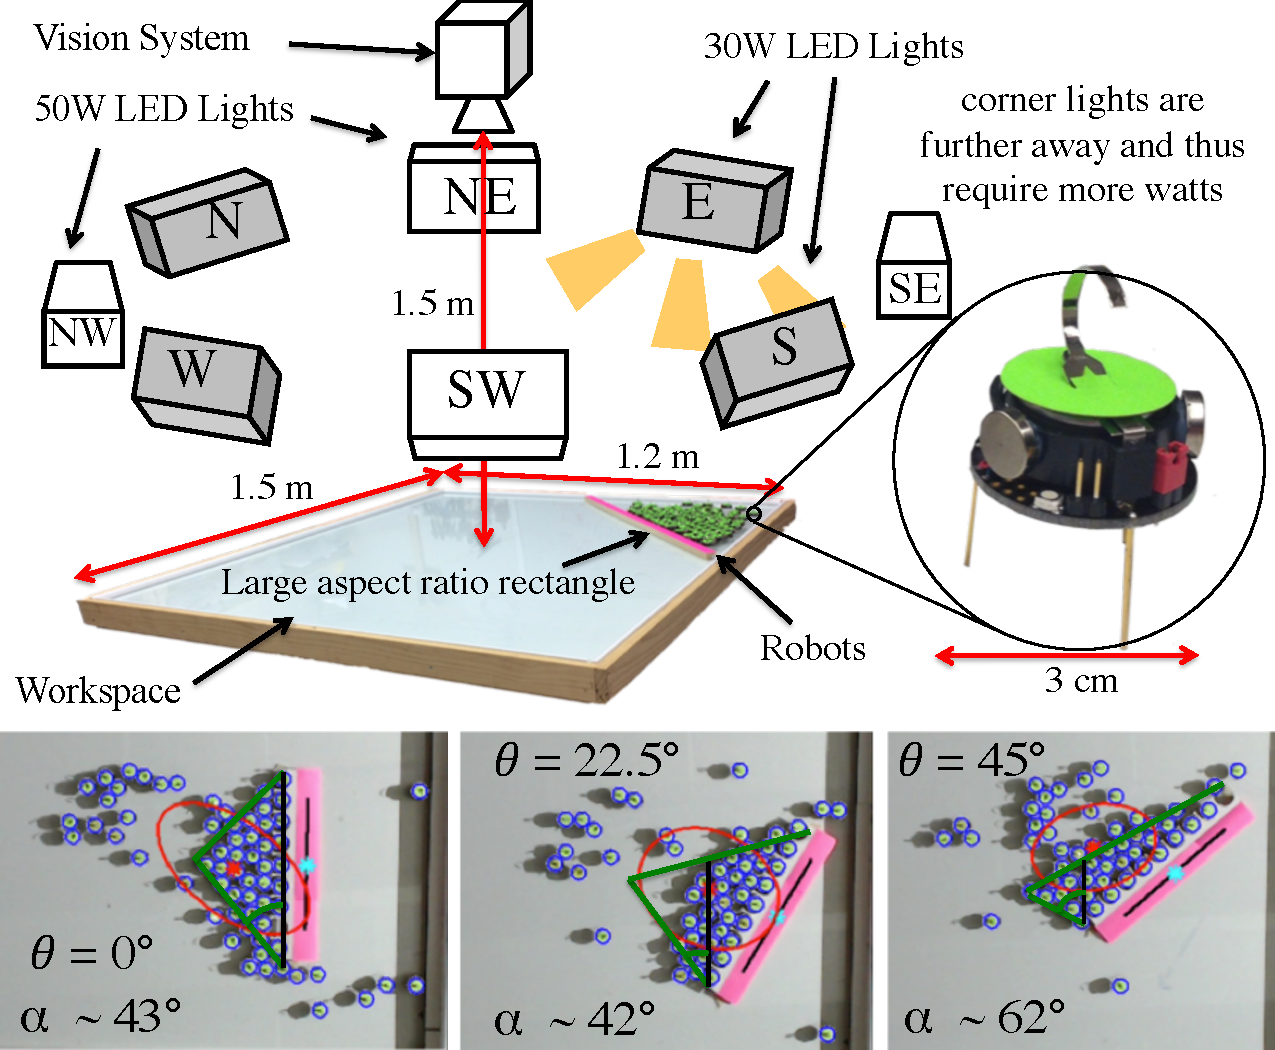
\includegraphics[width=.8\columnwidth]{SetUp.pdf}
\end{center}
%\vspace{-1em}
\caption{\label{fig:setup}
Hardware platform:  table with 1.5$\times$1.2 m workspace, surrounded by eight remotely triggered LED floodlights, with an overhead machine vision system.
}
%\vspace{-1.5em}
\end{figure}




%The experiments from Section \ref{sec:simulation}.a were manually demonstrated using this physical swarm.
%Fig. \ref{fig:expBig} illustrates an experiment showing pure torque control with a swarm of robots. In this figure a large-aspect-ratio rectangle  (91$\times$2 cm, colored pink in the image) was hinged to one side of the table.  Like a door, this object could only be moved around this pivot. 
%Two trials were performed.  In each trial the swarm was initialized in the lower right side of the table, and then commanded to push the object with the mean position of the swarm directed toward a point distance $C$ from the pivot point. Data was recorded for 150 seconds.
%In the first trial, $C = L$, so the robots were commanded to push the door at the extreme edge of the door from the pivot.  
%In the second trial $C = 1/2 L$, and so the swarm pushed the object in the center of the rectangle.
%As discussed in Section \ref{sec:simulation}, the robots spread when commanded to push the object at the extreme end, and half of the robots flowed past the end of the rectangle without engaging the rectangle.
% This illustrates a key difference between robotic swarms and a single pusher robot. The swarm exerts the most torque when  \eqref{eq:swarmtorque} is maximized.
%  \eqref{eq:swarmtorque} is maximized when the majority of the swarm engages the object.
%For this reason in Fig. \ref{fig:expBig}, the trial in the second row of screenshots moves the door further than the  trial in the  first row.






\begin{figure}
\begin{center}
	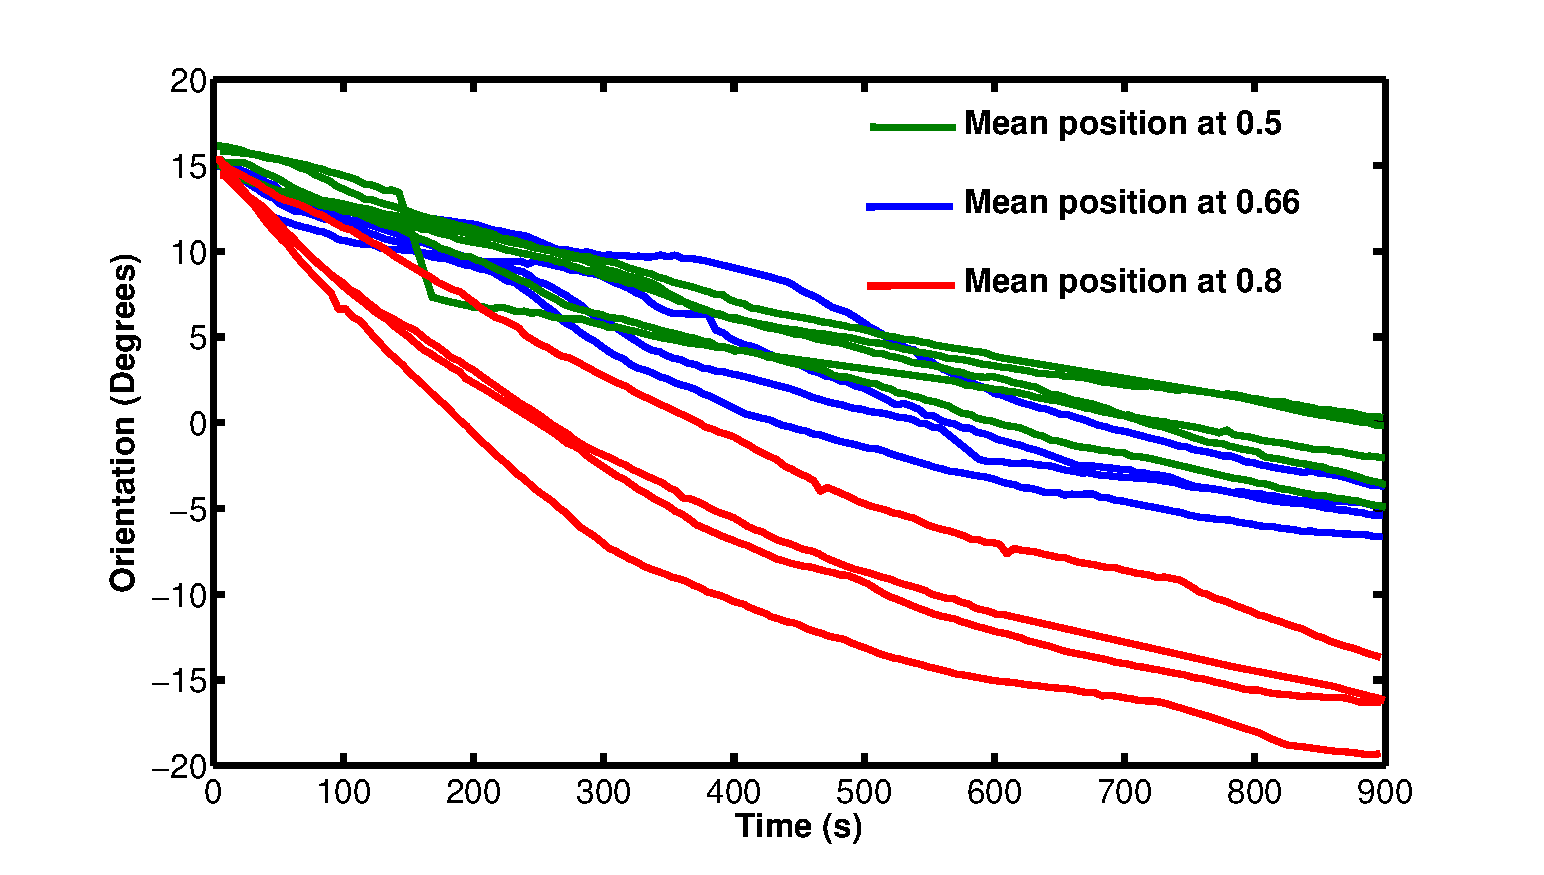
\includegraphics[width=\columnwidth]{ComparisonAllPivoted.eps}
\end{center}
%\vspace{-1em}
\caption{\label{fig:PivotedKilobot}
Pivoted object using uniformly distributed Kilobots with $\sigma = 0.05 L = \SI{6.8}{\centi \metre}$, but different mean positions. Mean positions are normalized along a rod of length 1.42 m.
}
%\vspace{-1.5em}
\end{figure}



The previous sections assumed perfect transmission of force from each particle to the object. 
Accurate swarm torque control is difficult.
In 2D, a swarm of $n$ particles has $2n$ degrees of freedom.  
The swarm, when steered toward an object, begins interacting with the object at different times. 
The number of particles touching this object as a function of time is difficult to predict and often impossible to directly measure.
Stochastic effects make long-term prediction challenging.
Even when it is possible to predict which particles will hit the object first, as particles interact with the object, the swarm's configuration changes.
The challenge is not only limited to swarm-object interaction, but also to swarm-swarm interactions when the swarm self-collides  or is split into multiple components. 
As a result, the force the swarm will exert on the object is not easy to predict. 
%Predicting the force a swarm exerts on an object requires knowing the location of every robot in contact with the object. 
To demonstrate the analytical results from Section \ref{sec:torqueDist} hold, we performed experiments using centimeter-scale hardware robots called \emph{Kilobots}.


%\subsection{Hardware System}


%Our experiments are on 
  These allow us to emulate a variety of dynamics, while enabling a high degree of control over robot function, the environment, and data collection. The Kilobot, from \cite{Rubenstein2012,rubenstein2014programmable}, is a low-cost robot designed for testing collective algorithms with large numbers of robots. It is available in an open source platform or commercially from~\cite{K-Team2015}.  Each robot is approximately 3 cm in diameter, 3 cm tall, and uses two vibration motors to move on a flat surface at speeds up to 1 cm/s.  Each robot has one ambient light sensor that is used to implement \emph{phototaxis},  moving towards a light source. 


%3 robots were donated to another lab during this test.
These experiments used up to $n = 97$ Kilobots, a glass-covered 1.5 m$\times$1.2 m whiteboard as the workspace, and 30 W and 50 W LED floodlights arranged 1.5 m above the plane of the table at the midpoint of the east side of a 6 m square centered on the workspace, as shown in Fig.~\ref{fig:setup}. Above  the table, an overhead machine vision system tracks the position of the swarm. For the last two experiments, we designed the object to rigidly hold the swarm, and programmed the robots to go straight. 

\subsection{Pushing a pivoted object}

Fig. \ref{fig:expBig} shows snapshots of the experiment for a pivoted object at different mean positions for the swarm when they are uniformly distributed. The object was designed such that the Kilobots keep the starting uniform distribution with $\sigma = 0.05 L = \SI{6.8}{\centi \metre}$. Kilobots were programmed to go straight so that they always apply force perpendicular to the object. The results of different mean positions are shown in Fig.~\ref{fig:PivotedKilobot} for four trials at $\mu=[0.5, 0.66, 0.8]$. Mean positions near the optimal solution of \eqref{eq:maxMuPivot} increase torque.


The experiments from Section \ref{sec:simulation}.a were manually demonstrated using this physical swarm.
Fig. \ref{fig:expBig} illustrates an experiment showing pure torque control with a swarm of robots. In this figure a large-aspect-ratio rectangle  (91$\times$2 cm, colored pink in the image) was hinged to one side of the table.  Like a door, this object could only be moved around this pivot. 
Two trials were performed.  In each trial the swarm was initialized in the lower right side of the table, and then commanded to push the object with the mean position of the swarm directed toward a point distance $C$ from the pivot point. Data was recorded for 150 seconds.
In the first trial, $C = L$, so the robots were commanded to push the door at the extreme edge of the door from the pivot.  
In the second trial $C = 1/2 L$, and so the swarm pushed the object in the center of the rectangle.
As discussed in Section \ref{sec:simulation}, the robots spread when commanded to push the object at the extreme end, and half of the robots flowed past the end of the rectangle without engaging the rectangle.
 This illustrates a key difference between robotic swarms and a single pusher robot. The swarm exerts the most torque when  \eqref{eq:swarmtorque} is maximized.
  \eqref{eq:swarmtorque} is maximized when the majority of the swarm engages the object.
For this reason in Fig. \ref{fig:expBigNormal}, the trial in the second row of screenshots moves the door further than the  trial in the  first row.


\begin{figure*}
\centering
\renewcommand{\figwid}{0.24\columnwidth}
\begin{overpic}[width =\figwid]{PivotedEnd1of4.pdf}%\put(1,55){a)}
\end{overpic}
\begin{overpic}[width =\figwid]{PivotedEnd2of4.pdf}
\end{overpic}
\begin{overpic}[width =\figwid]{PivotedEnd3of4.pdf}
\end{overpic}
\begin{overpic}[width =\figwid]{PivotedEnd4of4.pdf}
\end{overpic}\\
\vspace{0.5em}
\begin{overpic}[width =\figwid]{PivotedMiddle1of4.pdf}%\put(1,55){a)}
\end{overpic}
\begin{overpic}[width =\figwid]{PivotedMiddle2of4.pdf}
\end{overpic}
\begin{overpic}[width =\figwid]{PivotedMiddle3of4.pdf}
\end{overpic}
\begin{overpic}[width =\figwid]{PivotedMiddle4of4.pdf}
\end{overpic}
%\vspace{-1em}
\caption{\label{fig:expBig}{Snapshots showing the effect of pushing a pivoted rectangular object at different distances from the pivot point. 
%56 robots were programmed to move straight. The object is designed to maintain the initial distribution of the robots. 
%The top row of snapshots illustrate the swarm pushing at the end of the object.
 The top row shows the frames with the mean position is at 0.75 of the object length. The bottom row show frames with swarm mean position $\mu = 1/2$. %See attachment for experimental videos.
%\textcolor{red}{??Why are there 4 robots per row in the pictures but 3 robots per row in the closeup? }
 }
%\vspace{-2em}
}
\end{figure*}
\begin{figure*}
\centering
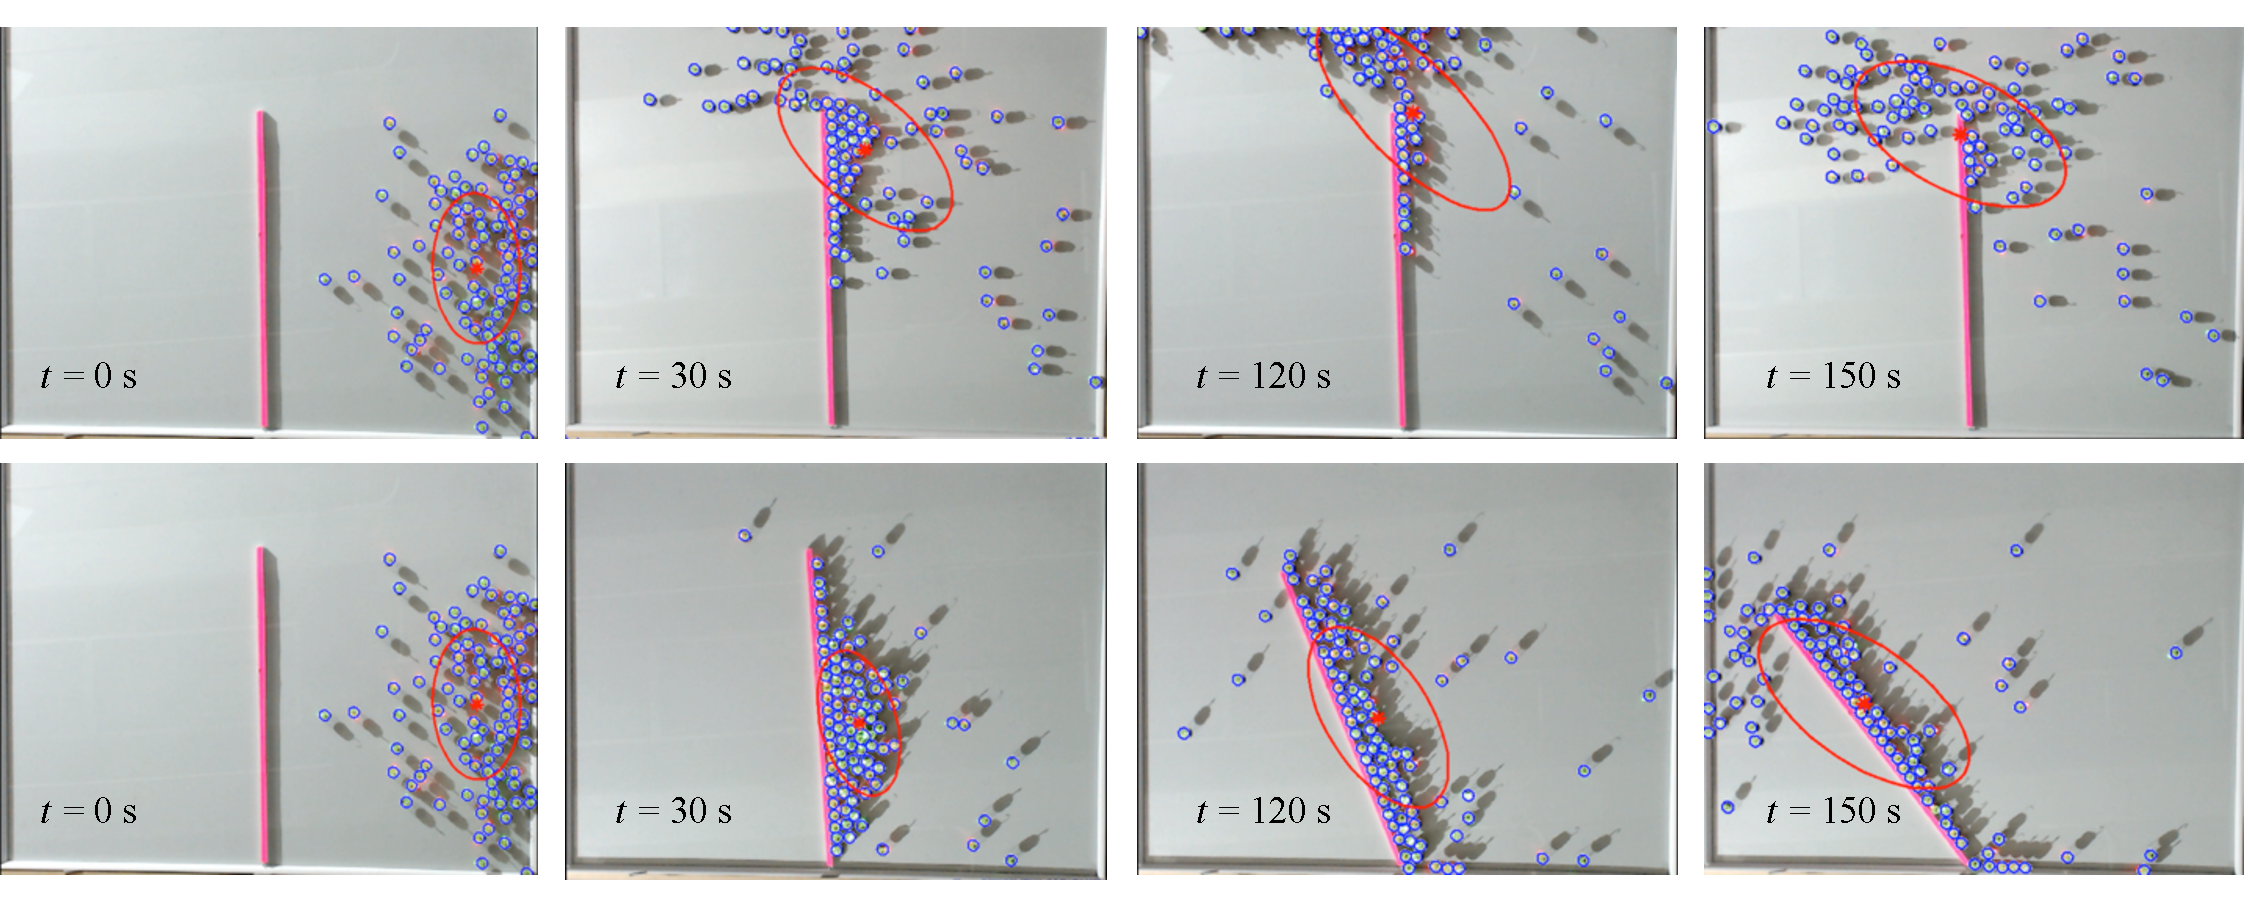
\includegraphics[width=\columnwidth]{Experiment.pdf}
\vspace{-1em}
\caption{\label{fig:expBigNormal}{Snapshots showing the effect of pushing a pivoted rectangular object at different distances from the pivot point. 
% 97 robots were programmed to move toward the brightest light in the room, and controlled by choosing which of 8 lights were on at any given instant.
 The top row of snapshots illustrate the swarm pushing at the end of the object.  %In this case,  the swarm flows past the object and the force decreases.
 The bottom row illustrates that when the swarm pushes at the middle of the object the force provided by the swarm remains constant.% In this case the swarm does not flow past the object. %See video attachment for recordings of these experiments~{\cite{ShahrokhiTorqueVideo}}.
%\textcolor{red}{??Can you get higher resolution? }
 }
%\vspace{-2em}
}
\end{figure*}

%%%%%%%%%%%%%%%%%%%%%%%%%%%%%%%%%%%%%%%
\subsection{Orientation control of a free object}

\begin{figure*}
\centering
\begin{overpic}[width =0.32\columnwidth]{orient1.png}\put(70,5){\emph{t} = 0 s}
\end{overpic}
\begin{overpic}[width =0.32\columnwidth]{orient3.png}\put(65,5){\emph{t} = 10 s}
\end{overpic}
\begin{overpic}[width =0.32\columnwidth]{orient2.png}\put(65,5){\emph{t} = 60 s}
\end{overpic}\\
\vspace{1em}
\begin{overpic}[width =0.32\columnwidth]{orient4.png}\put(65,5){\emph{t} = 90 s}
\end{overpic}
\begin{overpic}[width =0.32\columnwidth]{orient5.png}\put(65,5){\emph{t} = 120 s}
\end{overpic}
\begin{overpic}[width =0.32\columnwidth]{orient6.png}\put(65,5){\emph{t} = 150 s}
\end{overpic}
\caption{\label{fig:expOrient}{Snapshots showing orientation control of a free object using 97 hardware robots that all get the same control input. Light direction is the global control input and the robots are programmed to move toward the brightest light in the environment.
 }
%\vspace{-2em}
}
\end{figure*}
Figure \ref{fig:expOrient} shows snapshots of orientation control of a free rod using 97 Kilobots. Kilobots were programmed to move toward the brightest light in the room. Therefore, the light is the global input. The goal orientation of the object changed periodically, and the robots will go to a corner when the goal orientation is achieved. 

%\textcolor{Red}{TODO?? insert content from orientation control experiment, number of robots, timing, show a series of images, etc.}





